\documentclass{article}
\usepackage[utf8]{inputenc}
\usepackage{graphicx}


\renewcommand{\vec}[1]{
	\mathbf{#1}
}


\title{Theory of linear regression}
\date{\today}
\author{Chris Miles}

\begin{document}
	
	\maketitle
	
	\section{Overview}
	We are interested in predicting some output value $y$ from knowing a collection of input features $x_1, x_2, \dots x_n$ represented as a vector $\vec{x}= (x_1, x_2, \dots x_n)$. Suppose we have examples of the pair $(\vec{x}^{(k)}, y^{(k)})$ for $k = 1, 2,  \dots n$ that make up our dataset $D$ from which we would like to infer the relationship between $\vec{x}$ and $y$. This is the task of many supervised learning problems. Linear regression makes a number of assumptions about the relationship between $\vec{x}$ and $y$. 
	It models the relationship as
	\[\hat{y}(\vec{x} ; \vec{m}, b) = \vec{m}\cdot\vec{x} + b\]
	The goal is to fit parameters $\vec{m}$ and $b$ in the above equation to the dataset $D$ such that the values for $y^{(k)}$ and the predicted $\hat{y}^{(k)} = \vec{m}\cdot\vec{x}^{(k)} + b$ are close on average across all $k$. More specifically, linear regression fits $\vec{m}$ and $b$ through the following cost function:
	
	\[J(\vec{m}, b) = \frac{1}{n}\sum_{k = 1}^{n}|\hat{y}(\vec{x}^{(k)}; \vec{m}, b) - y^{(k)}|^2\]
	 which is the mean square error between the predicted $\hat{y}$ and the true value $y$ for each point. 
	 
%	 \section{Solvers}
%	 
%	 \subsection{Normal equation}
%	 
%	 \subsection{Gradient descent}
%	 
%	 \section{Time complexity}
%	 
%	 \section{Space complexity}
%	 
%	 \section{Overfitting and underfitting conditions}
%	 
%	 \section{Probabilistic interpretation and maximum likelihood estimation}
%		For example, we might be able to say something about the price of a house (output variable $y$) if we knew its square footage (input feature $\vec{x}$).
%
%	
%	where $\vec{m}$ is a vector of coefficients and $b$ is the intercept term or bias term. The probability distribution for the target variable $y$ is given by 
%	\[p(t|\vec{x}, \vec{w}, \sigma) = \mathcal{N}( t| \vec{w}\cdot \vec{x}, \sigma)\]
%	This is probability for single instance in the dataset.	
%	
%	% ADD MAXIMUM LIKELYHOOD DERIVATION
%	
%	% ADD SHOW DERIVATION OF NORMAL EQUATION FROM LEAST SQUARES COST
%	\begin{figure}
%		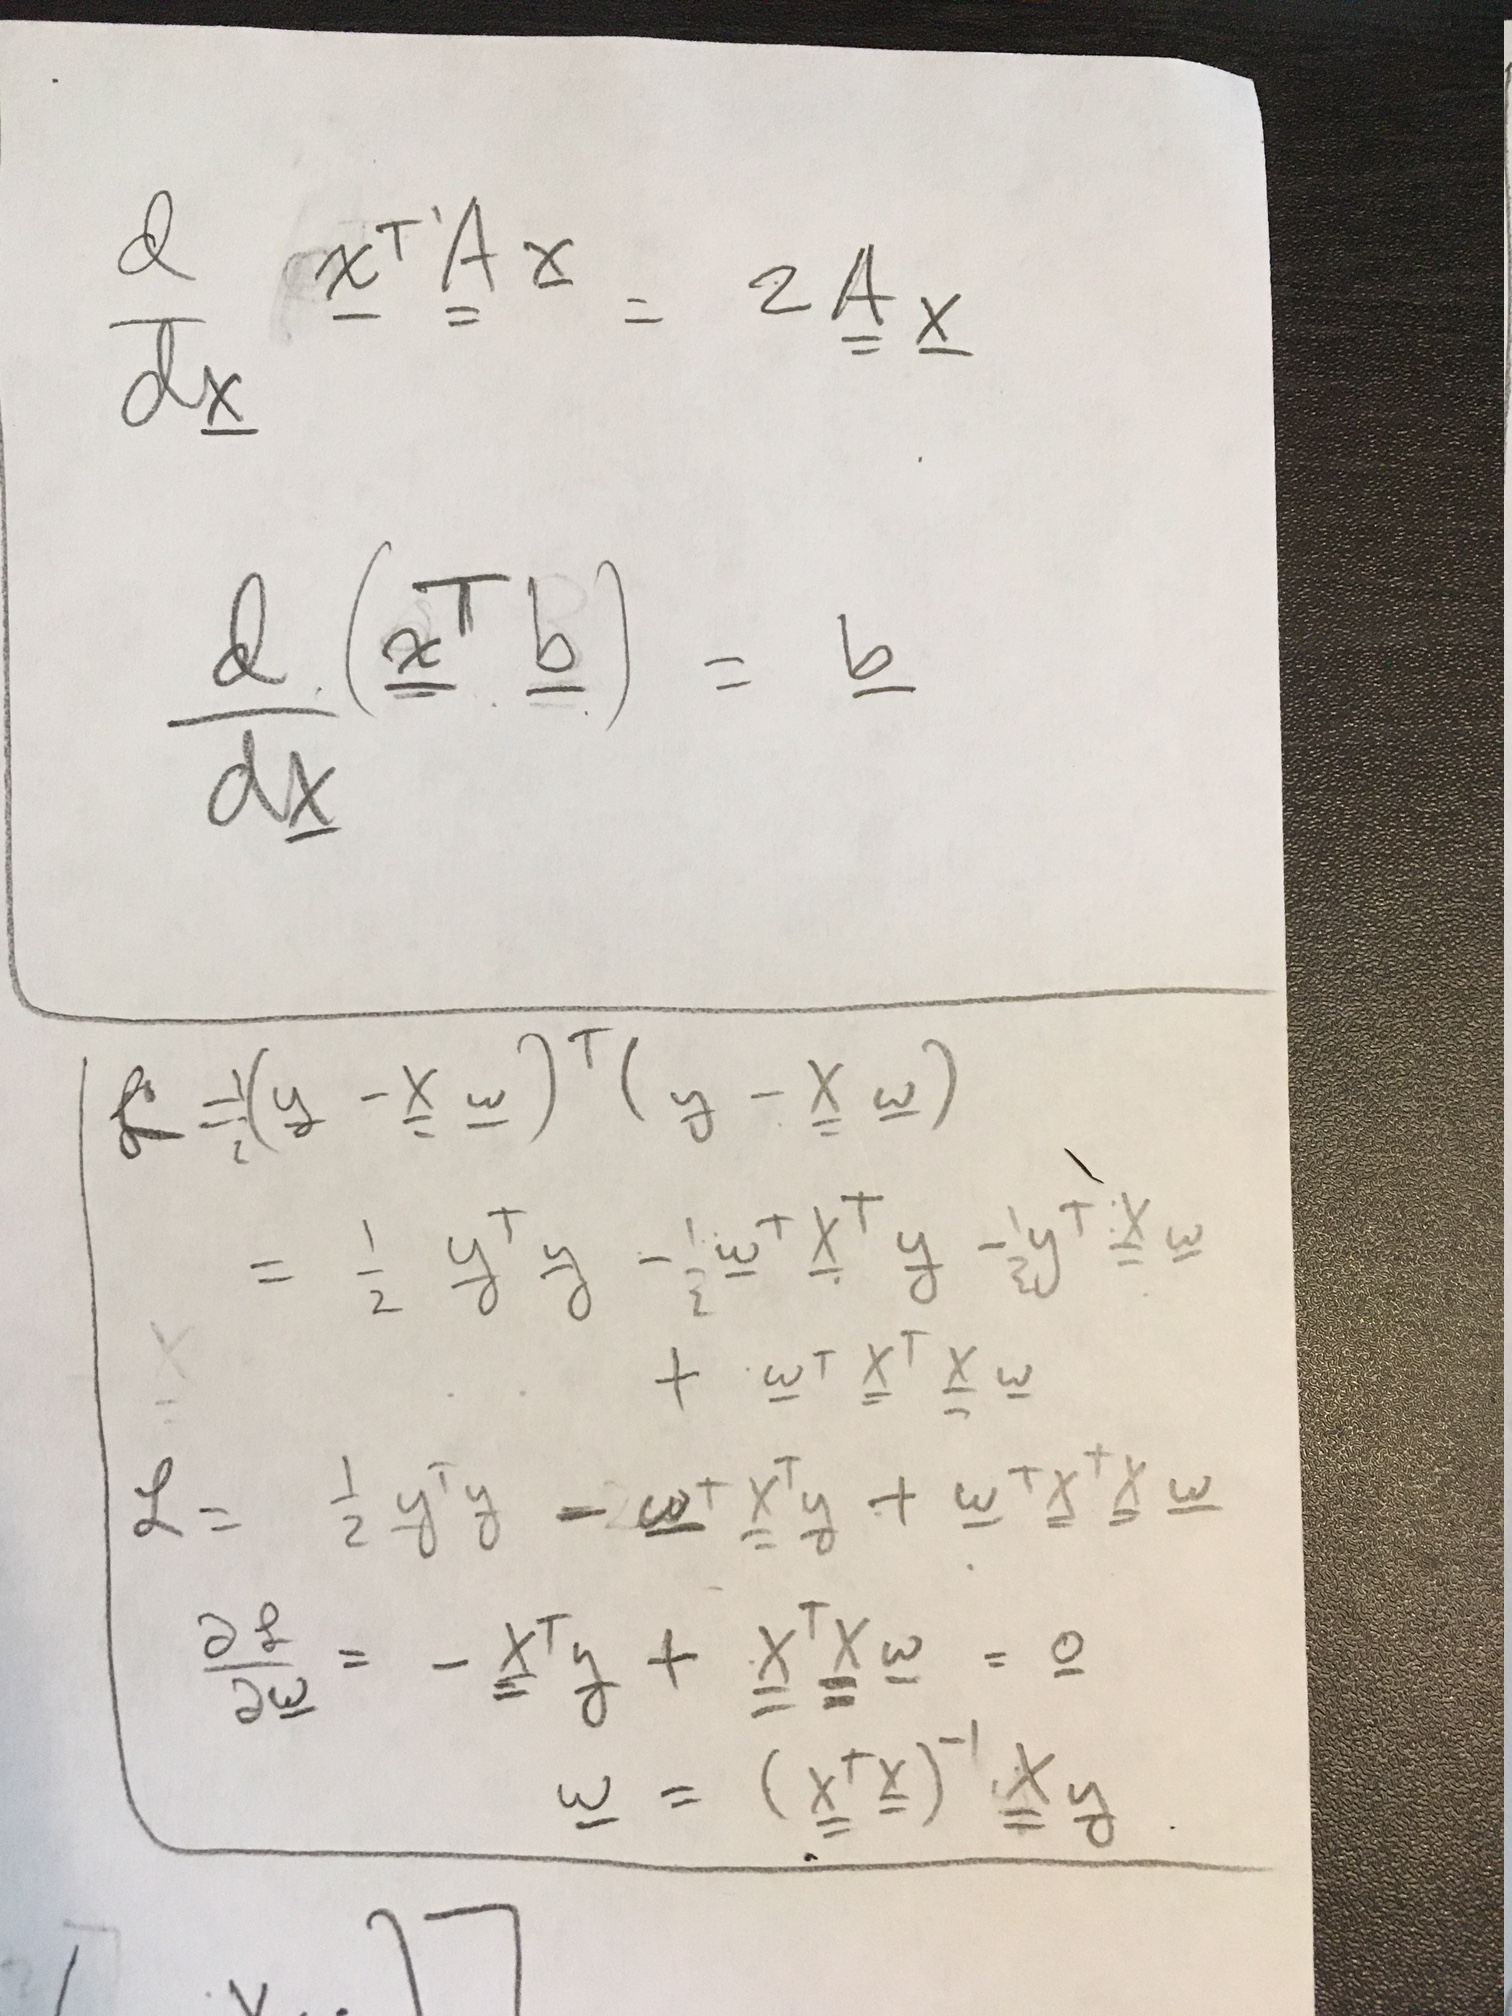
\includegraphics[width=0.5\textwidth]{images/linear-regression-normal-equation}
%	\end{figure}
%	
%	Normal equation is given by:
%
%	\[\vec{w} = (\vec{X}^T\vec{X})^{-1}\vec{X}^T\vec{y}\]


	
\end{document}